\documentclass[11pt]{report}
\usepackage{geometry}                % See geometry.pdf to learn the layout options. There are lots.
\geometry{letterpaper}                   % ... or a4paper or a5paper or ... 
%\geometry{landscape}                % Activate for for rotated page geometry
%\usepackage[parfill]{parskip}    % Activate to begin paragraphs with an empty line rather than an indent
\usepackage{graphicx}
\usepackage{amsmath}
\usepackage{amssymb}
\usepackage{epstopdf}
\DeclareGraphicsRule{.tif}{png}{.png}{`convert #1 `dirname #1`/`basename #1 .tif`.png}

\title{HProlog Manual}
\author{Tim Yates}

\begin{document}
\maketitle

\tableofcontents


%
% Overview
%

\chapter{About HProlog}

HProlog is a interpreter and compiler for a subset of Prolog. HProlog is written in Haskell. Its features include:

\begin{itemize}
\item Full and correct support for resolution of logical goals, including recursive rules and nested structures
\item Negation as a failure
\item A compiler targeting a simplified version of the \emph{Warren Abstract Machine} (WAM), as defined in Hasan Ait-Kaci's reconstruction\footnote{http://wambook.sourceforge.net/wambook.pdf}
\item Lists and numbers (but unfortunately no math at this point)
\item User-defined operators
\end{itemize}


%
% Usage
%

\chapter{Using HProlog}

\section{Setup}

HProlog is distributed as a \emph{cabal package},\footnote{http://www.haskell.org/cabal/} a commomly-used distribution system for Haskell programs. To build it, you will need to install the \textbf{Haskell Platform}.\footnote{http://hackage.haskell.org/platform/} Once that is installed, you can compile HProlog by running the following commands inside the directory where you unpacked the HProlog distribution:

\begin{verbatim}
$ cabal configure
$ cabal build
\end{verbatim}

After that, the HProlog binary will be located at \texttt{dist/build/prolog/prolog}. You can copy it into the base directory for convenience:

\begin{verbatim}
$ cp dist/build/prolog/prolog .
\end{verbatim}


\section{Usage}

When you first start HProlog, the program presents an interactive prompt where you can run queries and built-in commands:

\begin{verbatim}
$ ./prolog
?-
\end{verbatim}

You can read in files using the \emph{consult/1} command. Alternatively, you can specify files to consult through the command line:

\begin{verbatim}
$ ./prolog file1 file2
?-
\end{verbatim}

When you are finished with your session, press \emph{Control+D} to quit.


\section{Examples}

The following sections contain example sessions using the files provided in the \texttt{test/} directory.

\subsection{Family Tree Database}

\begin{verbatim}
$ cd test/
$ ../prolog
?- consult(family_trees).
true.
?- parent_child(bill, ted).
true.
?- parent_child(ted, bill).
false.
?- parent_child(Who, bob).
Who = bill ? ;

Who = mary ? ;

false.
?- ancestor_descendent(kim, Whom).
Whom = george ? ;

Whom = mary ? ;

Whom = ted ? ;

Whom = bob ? ;

false.
?- ancestor_descendent(Who, ted).
Who = bill ? ;

Who = mary ? ;

Who = george ? ;

Who = susan ? ;

Who = dave ? ;

Who = kim ? ;

false.
?- ^D
\end{verbatim}

\subsection{List Processing}

\begin{verbatim}
$ cd test/
$ ../prolog
?- consult(lists).
true.
?- member(What, [a,b,c]).
What = a ? ;

What = b ? ;

What = c ? ;

false.
?- append([a,b,c], [d,e,f], What).
What = [a,b,c,d,e,f] ? ;

false.
?- append(What, [d,e,f], [a,b,c,d,e,f]).
What = [a,b,c] ? ;

false.
?- reverse([a,b,c,d]).
What = [d,c,b,a] ? ;

false.
?- ^D
\end{verbatim}

\subsection{Compiling}

\begin{verbatim}
$ cd test/
$ ../prolog
?- consult(lists).
true.
?- consult(family_trees).
true.
?- consult(crazy_structures).
true.
?- compile(everything).
true.
?- ^D
\end{verbatim}

At the end of this session, there should be a file named \texttt{everything.wam} in the \texttt{test/} directory. It will contain WAM instructions in text format for all the predicates defined in all three test files.


\section{Tests}

Aside from the examples given above, HProlog also has unit tests for its parser and unification engine. To run these tests (from within the main HProlog directory):

\begin{verbatim}
$ ghci -isrc
GHCi, version 7.0.3: http://www.haskell.org/ghc/  :? for help
Loading package ghc-prim ... linking ... done.
Loading package integer-gmp ... linking ... done.
Loading package base ... linking ... done.
Loading package ffi-1.0 ... linking ... done.
Prelude> :load Prolog.Test
[1 of 5] Compiling Prolog.Data      ( src/Prolog/Data.hs, interpreted )
[2 of 5] Compiling Prolog.Parser    ( src/Prolog/Parser.hs, interpreted )
[3 of 5] Compiling Prolog.Compiler  ( src/Prolog/Compiler.hs, interpreted )
[4 of 5] Compiling Prolog.Interpreter ( src/Prolog/Interpreter.hs, interpreted )
[5 of 5] Compiling Prolog.Test      ( src/Prolog/Test.hs, interpreted )
Ok, modules loaded: Prolog.Test, Prolog.Data, Prolog.Parser, Prolog.Interpreter, Prolog.Compiler.
*Prolog.Test> runTestTT test_parser
Loading package transformers-0.2.2.0 ... linking ... done.
Loading package bytestring-0.9.1.10 ... linking ... done.
Loading package mtl-2.0.1.0 ... linking ... done.
Loading package parsec-3.1.1 ... linking ... done.
Loading package HUnit-1.2.2.3 ... linking ... done.
Loading package array-0.3.0.2 ... linking ... done.
Loading package containers-0.4.0.0 ... linking ... done.
Cases: 29  Tried: 29  Errors: 0  Failures: 0
Counts {cases = 29, tried = 29, errors = 0, failures = 0}
*Prolog.Test> runTestTT test_unification
Cases: 17  Tried: 17  Errors: 0  Failures: 0
Counts {cases = 17, tried = 17, errors = 0, failures = 0}
*Prolog.Test> :quit
Leaving GHCi.
\end{verbatim}

\textbf{Note}: As of this writing, there is a bug in operator parsing that will fail one of the parser tests. The only problem the bug causes is an inability to enforce non-associativity of operators. It should be fixed, but for now, it won't cause any problems in normal usage of the program.



%
% Technical Description
%

\chapter{Technical Description}

\section{Architecture}

\begin{figure}[htb]
\centering
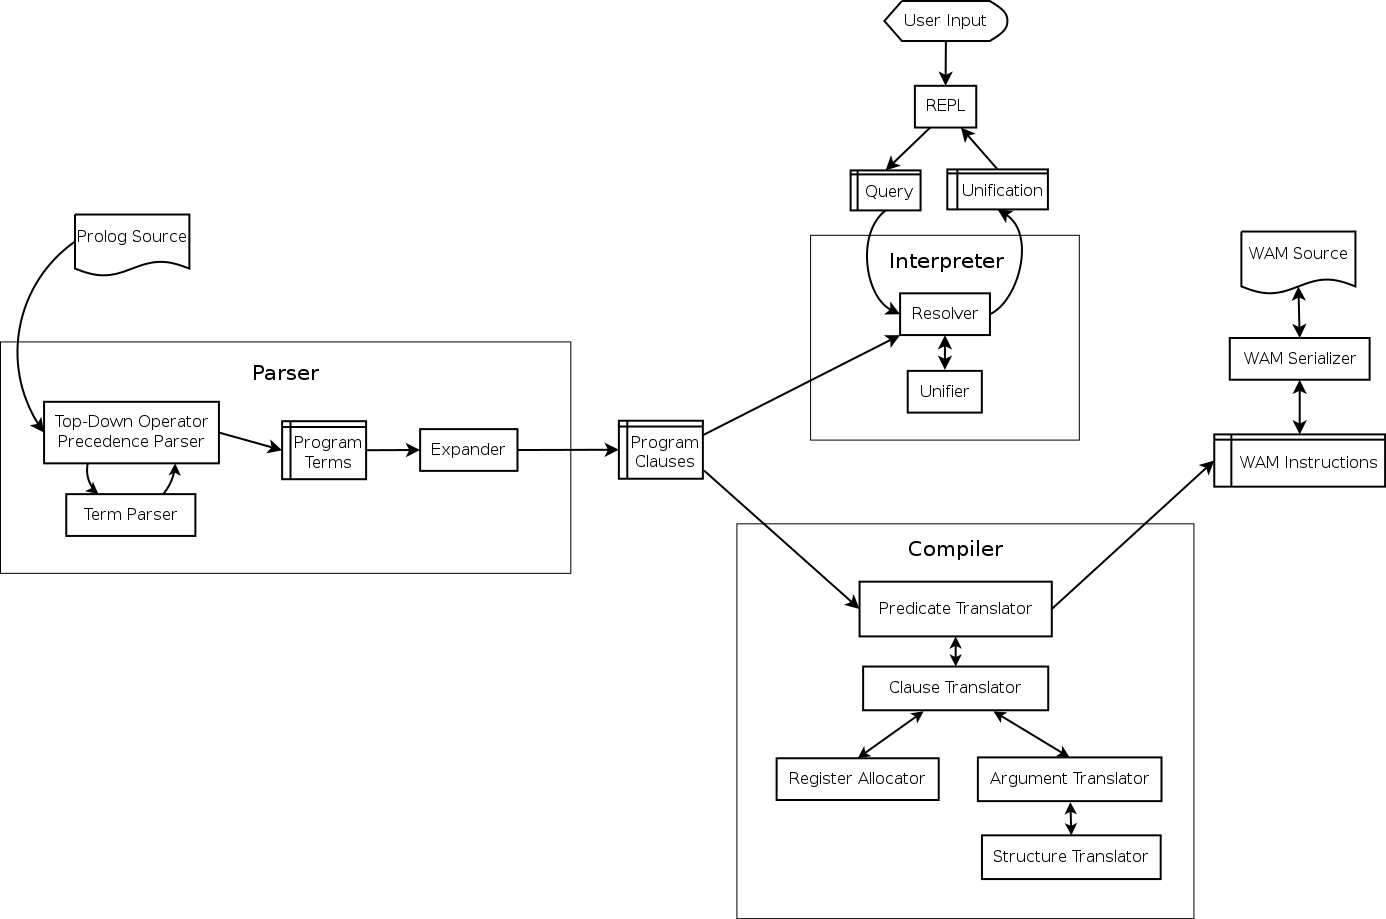
\includegraphics[width=\linewidth]{Architecture.png}
\caption{
  \textbf{Architecture diagram}. This version is slightly simplified. The interpreter is actually involved in parsing program clauses, so that directives in the source file (such as \emph{op/3} definitions and \emph{consult/1} directives) can be executed as they are read. Also, the compiler is run by the interpreter as a built-in predicate. The internal architectures are still accurate.
}
\label{fig:architecture}
\end{figure}

HProlog is roughly divided into a parser, interpreter, and compiler units as shown in Figure \ref{fig:architecture}. The job of each of these units is described in the following sections.


\section{Parser}

The parser is defined in \texttt{src/Prolog/Parser.hs}. Its job is to transform the concrete representation of Prolog rules into a list of rule data structures. We can divide this task into two levels: parsing rules, and parsing terms.

\subsection{Rules}

Consider the following input:
\begin{verbatim}
foo(X) :- bar(X, Y).
foo(a).
bar(Z, Z).
\end{verbatim}
This will be transformed into a list of data structures of the form:
\[
\mathbf{DefiniteClause} \; h \; [g_1, g_2, \ldots, g_n],
\]
where $h$ is the representation of the head of the clause, and $g_n$ is the representation of goal $n$ in the body. Facts (heads with no body) are represented in the same form, but the list of goals is empty.

Queries and directives (rules with no heads) are represented in the form:
\[
\mathbf{GoalClause} \; [g_1, g_2, \ldots, g_n].
\]

\subsection{Terms}

The next problem is how to represent the terms in the head and body of rules themselves. A \emph{term} is one of:
\begin{itemize}
\item An \emph{atom}: \texttt{a}, \texttt{foo}, \texttt{`with Quotes!'}, \texttt{-->}
\item A \emph{variable}: \texttt{X}, \texttt{SomeVar}
\item A \emph{number}: \texttt{123}
\item A \emph{compound term}: \texttt{f(a,b)}, \texttt{p(X, h(f(a), b))}
\end{itemize}
These are represented in the following forms:
\begin{itemize}
\item $ \mathbf{Atom}\; a $
\item $ \mathbf{Variable}\; v $
\item $ \mathbf{Number}\; n $
\item $ \mathbf{CompoundTerm}\; f \; [t_1, t_2, \ldots, t_n] $
\end{itemize}
where:
\begin{itemize}
\item $a$, $v$, and $f$ are the string representations of the atom, variable, and functor, respectively,
\item $n$ is the integer represented by the number token, and
\item $t_n$ is the $n$th subterm of the compound term.
\end{itemize}
Because compound terms contain other terms, the overall structure of parsed terms is a tree.

A final issue is how to deal with operators. HProlog supports user-defined operators, which are simply functors of arity 1 or 2 that are written in prefix, postfix, or infix notation. For example, the expression \texttt{a :- b} is really a compound term with functor \emph{:-/2}, and can also be written as \texttt{:-(a, b)}. HProlog uses a \emph{top-down operator precedence parser} to parse operations, which are then transformed into their term representation.


\section{Interpreter}

The interpreter is defined in \texttt{src/Prolog/Interpreter.hs}. Its job is to find logical solutions to queries using rules defined in a program. For example, consider the program:
\begin{verbatim}
parent_child(bill, ted).
parent_child(bill, bob).
parent_child(mary, ted).
parent_child(mary, bob).
parent_child(george, mary).
parent_child(susan, mary).

female(mary).
female(susan).
male(bill).
male(ted).
male(bob).
male(george).

mother_child(Mother, Child) :- female(Mother), parent_child(Mother, Child).
father_child(Father, Child) :- male(Father), parent_child(Father, Child).
\end{verbatim}
Some queries that could be performed on this program include:
\begin{itemize}
\item \verb|?- mother_child(susan, ted).| -- Is \texttt{susan} the mother of \texttt{ted}?
\item \verb|?- father_child(Who, mary).| -- \texttt{Who} is the father of \texttt{mary}?
\end{itemize}
To properly match these queries to rules in the program, we need two pieces: unification and resolution.

\subsection{Unification}

Unification is the process of substituting variables in two terms so that they match. For instance, \texttt{f(X, b)} can be unified with \texttt{f(g(a), Y)} by setting $X = g(a)$ and $Y = b$, so that both terms are equal to \texttt{f(g(a), b)}.

Unification is essentially the process of walking two term trees simultaneously and matching variables in one tree to the corresponding term in the other tree. We also have to obey a few rules:
\begin{itemize}
\item A variable can only have one substitution. We cannot unify \texttt{f(X, X) $\sim$ f(a, b)}, because that would require setting $X = a$ and $X = b$ at the same time.
\item Only variables can be substituted. We cannot unify \texttt{f(a) $\sim$ f(b)} by substituting $a = b$.
\item A variable cannot unify with a compound term that it occurs in (\emph{occurs check}). We cannot unify \texttt{X $\sim$ f(a, X)}, because that would produce a cyclic term.
\end{itemize}

In many cases, unification is impossible, so we have to handle failure appropriately.

\subsection{Resolution}

The heart of Prolog is \emph{resolution}. Resolution is an logical inference rule that can be used to solve the satisfiability problem for Horn formulas.

Consider a query:
\begin{verbatim}
?- g1, g2, ..., gn.
\end{verbatim}
where $g_n$ are independent goals in the query. We can determine whether all the goals are true by trying to prove any of them wrong. If none of them can be proved wrong, then they are all true. Turning this into logical form:
\begin{align*}
& \neg(g_1 \wedge g_2 \wedge \ldots \wedge g_n) \\
=\; &\neg g_1 \vee \neg g_2 \vee \ldots \vee \neg g_n
\end{align*}

Now assume we have a rule:
\begin{verbatim}
g1 :- h1, h2, ..., hn
\end{verbatim}
We can represent this in logical form as:
\begin{align*}
& g_1 \leftarrow h_1 \wedge h_2 \wedge \ldots \wedge h_m \\
=\; & g_1 \vee \neg (h_1 \wedge h_2 \wedge \ldots \wedge h_m) \\
=\; & g_1 \vee \neg h_1 \vee \neg h_2 \vee \ldots \vee \neg h_m
\end{align*}

If we assume that both our goal and this rule are true, then we have:
\begin{align*}
& (g_1 \vee \neg h_1 \vee \neg h_2 \vee \ldots \vee \neg h_m) \wedge (\neg g_1 \vee \neg g_2 \vee \ldots \vee \neg g_n) \\
=\; & (g_1 \vee \neg (h_1 \wedge h_2 \wedge \ldots \wedge h_m)) \wedge (\neg g_1 \vee \neg (g_2 \wedge \ldots \wedge g_n))
\end{align*}
Now notice that if $g_1$ is true, then $\neg g_1$ would be false and $\neg (g_2 \wedge \ldots \wedge g_n)$ would have to be true. If $g_1$ were false, then $\neg (h_1 \wedge \ldots \wedge h_n)$ would have to be true. In other words, one of the non-$g_1$ terms must be true no matter what $g_1$ is, so we can eliminate $g_1$ altogether and get:
\begin{align*}
& \neg (h_1 \wedge h_2 \wedge \ldots \wedge h_m) \wedge \neg (g_2 \wedge \ldots \wedge g_n) \\
=\; & \neg h_1 \vee \neg h_2 \vee \ldots \vee \neg h_m \vee \neg g_2 \vee \ldots \vee \neg g_n
\end{align*}
This last step is ``resolution" proper. We now have a \emph{new} set of goals, and we can repeat the procedure on this new set. We repeat until we either eliminate all the variables, proving our negation false and the original goals true, or until we have no rules left to resolve with, proving our negation true and the original goals false.

In summary, the steps of resolution are:
\begin{enumerate}
\item Negate the original goal clause.
\item Find a rule to unify with. If no rules unify, then fail.
\item Resolve against that rule to generate a new goal clause.
\item If nothing is left, succeed. Otherwise, repeat from step 2.
\end{enumerate}

This is the basic algorithm used by HProlog, except that it also has to deal with the question of which rule to unify with when there are several possible alternatives. It handles this by (lazily) taking all possible paths and concatenating all the results into a single list. The result takes the same space complexity as so-called ``backtracking" algorithms, but in a much more straightforward manner.


\section{Compiler}

The compiler is defined in \texttt{src/Prolog/Compiler.hs}. Its job is to take the rules in a program and translate them to a series of instructions for the Warren Abstract Machine (WAM). The details of the WAM are much too complicated to lay out here, but they can be found in \emph{Warren's Abstract Machine: A Tutorial Reconstruction} by Hasan Ait-Kaci.\footnote{http://wambook.sourceforge.net/wambook.pdf} The version of the WAM targeted by HProlog is the one laid out in chapters 1-3 of that book. It does not include the many optimizations in chapter 4.

A simplified view of the job of the compiler is to take the rules and define them as callable procedures. These procedures are passed arguments through predefined registers. A rule of the form:
\begin{verbatim}
p(a1, a2, ..., an) :- q1(b1, b2, ..., bm), q2(...), ..., qn(...).
\end{verbatim}
does the following:
\begin{enumerate}
\item Allocate space on the stack to store variables
\item Extract the arguments $a_1, \ldots, a_n$ of $p/n$ and pull them onto the stack.
\item Pull the arguments $b_1, \ldots, b_m$ of $q_1/m$ from the stack and put them in registers, and call $q_1/m$
\item Do the same for the rest of the goals.
\end{enumerate}

While arguments, which contain references to terms in memory, are being moved from the stack to registers, their values are being unified. If unification fails, the whole rule fails. If more rules are possible, then the machine will try the other alternatives.

The compiler has to determine the right instructions in the right order to make this happen. Some examples of instructions are:
\begin{verbatim}
allocate 5
get_variable Y4 A1
get_value Y4 A2
put_variable Y3 A2
put_structure f/2 A3
unify_value X4
unify_value Y2
deallocate
\end{verbatim}
where terms like $X1$, $A2$, and $Y4$ denote temporary registers, argument registers, and stack locations, respectively.

Some of the complications the compiler has to deal with include:
\begin{itemize}
\item Assigning variables (and partially constructed structures) to appropriate registers.
\item Deciding whether to keep variables in the stack or in temporary registers.
\item Ordering the construction of nested terms so that they are constructed before the terms that contain them.
\end{itemize}




%
% Reference
%

\chapter{Reference}

The following built-in commands are available for you to use in HProlog:

\begin{description}

\item [consult(+Filename)]  \hfill \\
Read the Prolog source file \emph{``\textless{}Filename\textgreater{}.pl"} into the current session.

\item [compile(+Filename)]  \hfill \\
Compile all the predicates defined in the current session into WAM code, and dump the compiled output to \emph{``\textless{}Filename\textgreater{}.wam"}.

\item [not Goal]  \hfill \\
Negation as a failure: try to resolve \emph{Goal}. Fail if a resolution is found, otherwise succeed.

\item [true]  \hfill \\
Succeed without triggering any unification.

\item [fail]  \hfill \\
Fail the current rule immediately.

\item [op(+Precedence, +Type, +Symbol)]  \hfill \\
Define a new operator \emph{Symbol} with precedence \emph{Precedence} and fixity and associativity defined by \emph{Type}. Valid values for \emph{Type} are:

\begin{description}
\item [fx]  A non-associative prefix operator.
\item [fy]  A right-associative prefix operator.
\item [xf]  A non-associative postfix operator.
\item [yf]  A left-associative prefix operator.
\item [xfx]  A non-associative infix operator.
\item [xfy]  A right-associative infix operator.
\item [yfx]  A left-associative infix operator.
\end{description}

\end{description}



\end{document}  